\section{Is Multitask Deep Learning Practical for Pharma?}

This chapter is adapted from: 

Ramsundar, Bharath, Bowen Liu, Zhenqin Wu, Andreas Verras, Matthew Tudor, Robert P. Sheridan, and Vijay Pande. "Is multitask deep learning practical for pharma?." Journal of chemical information and modeling. \cite{ramsundar2017multitask}.

I was the first author and worked on conception of the original idea, implementation and execution of experiments, and writing of the paper.



\subsection{Abstract}
Multitask deep learning has emerged as a powerful tool for computational drug discovery. However, despite a number of preliminary studies, multitask deep networks have yet to be widely deployed in the pharmaceutical and biotech industries. This lack of acceptance stems from both software difficulties and from lack of understanding of the robustness of multitask deep networks. Our work aims to resolve both of these barriers to adoption. We introduce a high-quality open-source implementation of multitask deep networks as part of the DeepChem open-source platform. Our implementation enables simple python scripts to construct, fit, and evaluate sophisticated deep models. We use our implementation to analyze the performance of multitask deep networks and related deep models on four collections of pharmaceutical data (three of which have not previously been analyzed in the literature). We split these datasets into train/valid/test using time and neighbor-split to test multitask deep-learning performance under challenging conditions. Our results demonstrate that multitask deep networks are surprisingly robust and can offer strong improvement over random forests. Our analysis and open-source implementation in DeepChem provide an argument that multitask deep-networks are ready for widespread use in commercial drug discovery. 


\subsection{Introduction}
Deep learning has had unprecedented impact on computer science and technology over the last five years. The advent of sophisticated deep models has enabled the construction of powerful visual, speech, and natural language understanding systems \cite{lecun2015deep}. Over the past few years, deep learning has begun to influence drug discovery. In 2012, MSD (Merck \& Co., Inc., Kenilworth, NJ USA) hosted a Kaggle contest to measure the ability of data-science to improve predictive accuracies of quantitative structure-activity relationship (QSAR) methods. The winning entry used multitask deep networks (ensembled with other machine-learning techniques) to achieve a 15\% relative improvement over the baseline \cite{DahlKaggle}. In follow-up work, MSD demonstrated that strong improvements could be 
achieved on the Kaggle datasets using a single deep learning architecture, without constructing ensemble models \cite{ma2015deep}. In parallel, other research has demonstrated that large scale multitask deep networks can yield strong improvements over singletask models on public datasets with hundreds of tasks, extending MSD's work with smaller dataset collections \cite{ramsundar2015massively,unterthiner2014deep}. Similarly, recent work from Vertex demonstrates that multitask deep networks can offer improvements over simpler methods for modeling ADMET (absorption, distribution, metabolism, excretion, and toxicity) datasets \cite{kearnes2016modeling}. 

However, despite significant preliminary research, deep multitask networks have not succeeded in achieving broad adoption in the pharmaceutical and biotechnology industries. Transforming a machine-learning based research prototype into a production system can present
many challenges. For example, the winning entry for Netflix's million dollar recommendation challenge was not actually deployed in Netflix's production system due to engineering costs \cite{netflixNever}. Parts of the solution (singular value decompositions and restricted Boltzmann machines) were deployed, but shifting customer requirements rendered the full solution too unwieldy for broad implementation \cite{netflixBlog}.

Similar challenges may well be slowing the broad adoption of multitask deep networks in the pharmaceutical industry. Drug discovery companies often don't have strong software development teams, and creating a high-quality multitask deep network implementation is a formidable software engineering challenge. Each piece of research cited above uses an independent multitask implementation. While a research team may be able to create custom deep-learning implementations, such feats remain challenging for industrial teams. Until recently, a similar situation held more broadly within the deep learning community. While research teams could implement deep-learning systems, industrial users often stayed away due to the engineering challenges. However, this situation changed dramatically with the advent of sophisticated open source deep learning frameworks such as Tensorflow, Theano, and Keras \cite{abadi2016tensorflow,bastien2012theano,chollet2015keras}. These platforms offer convenient software primitives for building sophisticated deep architectures with low-overhead. As a result, the adoption of deep-learning techniques by the software industry has increased accordingly.

While deep learning systems offer powerful conveniences for users, the native
%comment MT: replace raw with native
packages are not well-suited to handle chemical datasets. Data loading procedures don't support common chemical formats such as SMILES strings \cite{weininger1988smiles} or provide for data-splits based on chemical scaffolds \cite{bemis1996properties}. The DeepChem library developed at Stanford provides a wrapper around Tensorflow that understands and facilitates the processing of chemical datasets \cite{deepchem}. DeepChem has been used for both application projects (modeling inhibitor design for BACE-1 \cite{subramanian2016computational}) and for algorithmic development (of novel one-shot deep-learning techniques for drug discovery \cite{altae2017low}).

In this work, we introduce a high-quality multitask deep network implementation to DeepChem. We use this implementation to construct multitask models on four broad collections of pharmaceutical data. We start by using DeepChem's implementation to reproduce results on the Kaggle collection explored by MSD previously. We then construct multitask deep models on the Factors, Kinase, and UV dataset collections from MSD (previously not analyzed in the literature). We aim to investigate whether multitask deep-learning is a robust tool; one that provides strong results across broad collections of pharmaceutical data.

We focus our analysis on gauging whether multitask networks provide consistent improvements over random-forest baselines. In particular, we aim to answer the question of whether deep networks can replace random-forest models without causing significant failures on a subset of predictive models. Furthermore, due to the ease of implementing new deep-learning architectures in DeepChem, we test the performances of two alternate deep learning architectures on these datasets. Google's Deepmind recently proposed progressive neural networks as a suitable architecture for solving sequences of challenging learning tasks \cite{rusu2016progressive} while leveraging transfer learning and avoiding learning failures. Progressive networks require an ordering of learning tasks (often unnatural in a drug-discovery setting with a collection of assays), so we also consider a variant bypass architecture halfway between multitask networks and progressive networks. Our analysis reveals that while these alternative architectures offer reasonable results, the simple multitask deep architecture currently remains the most robust deep architecture for QSAR datasets. On average, multitask deep networks offer performance boosts over random forest methods, but the improvements are not yet across the board.

To encourage adoption of multitask deep-learning methods, we open source all modeling code and datasets for the Kaggle, Factors, Kinase, and UV dataset collections as part of the DeepChem example suite. We hope that this example code and data will facilitate broader adoption of multitask deep-learning techniques for commercial drug discovery.

\subsection{Multitask Deep Learning with DeepChem}
\begin{figure}
  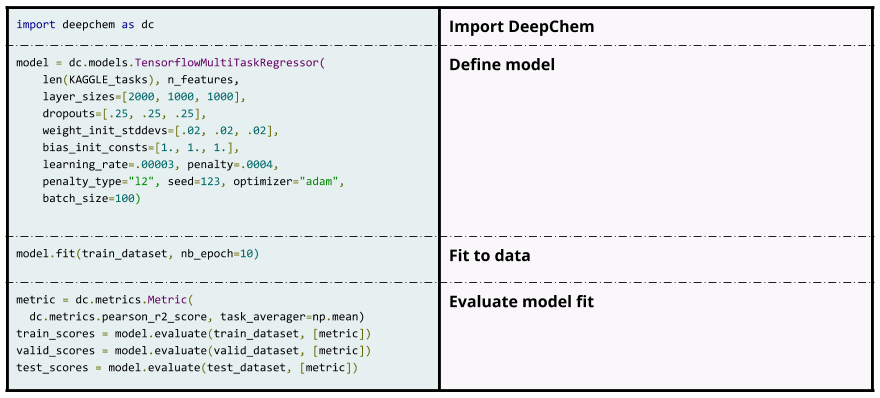
\includegraphics[width=\textwidth]{Images/deepchem_code.png}
  \caption{Example code for defining, training, and evaluating multitask deep networks for the Kaggle dataset with DeepChem. Code example is nearly complete, except for loading code. Full code for building networks on Kaggle datasets is available online}
  \label{fig:code}
\end{figure}

DeepChem offers a python API for constructing multitask deep-learning models. The API is object-oriented and modeled on the interfaces for popular machine-learning packages such as Scikit-Learn \cite{pedregosa2011scikit} and Keras \cite{chollet2015keras}. As part of this work, we contribute a high quality multitask deep network implementation to DeepChem.
%comment MT: DeepChem
Users can build, train, and evaluate multitask deep networks with simple python scripts.

Figure~\ref{fig:code} provides an (almost complete) code sample for using the multitask deep learning API in DeepChem to build a model for the Kaggle data collection. Users can specify model hyperparameters in the constructor for the multitask deep network. Figure~\ref{fig:code} demonstrates how a three hidden layer deep network, with dropout \cite{srivastava2014dropout} and $L^2$ regularization can be specified. Calling the \texttt{fit()} method fits the model using the ADAM optimization algorithm \cite{kingma2014adam} for 10 epochs over the training dataset. Note that code in 
%comment MT: add 'code in'
Figure~\ref{fig:code} has a \texttt{seed} flag for deep models. This flag allows multitask deep networks to be constructed in DeepChem with fixed random seed. Otherwise, model performance may vary on the order of a few percent due to random initialization choice, making debugging and model optimization challenging. Calling the \texttt{evaluate()} method allows users to evaluate the model using the squared Pearson correlation coefficient.

The full example for the Kaggle dataset is only slightly longer and has been open-sourced as part of the DeepChem example suite.

\subsection{Datasets}

\subsubsection{Data Description}
Modeling was performed on four collections of assays from MSD (see Table~\ref{tab:datasets} for details). The Kaggle collection is a collection of 15 of enzymatic inhibition and ADME/Tox datasets \cite{ma2015deep} with about 100,000
unique compounds. Not every compound in the Kaggle collection is tested against every assay. The Factors collection measures about 1500 of MSD's in-house compounds for IC50 of inhibition on 12 serine proteases, some of which are blood-clotting factors. The Kinase colection contains about 2500 in-house compounds measured for IC50 of inhibition on 99 protein kinases, carried out by a contract research partner. The UV collection tests 10,000
compounds on 190 absorption wavelengths, between 210 and 400 nanometers.

Pre-computed AP,DP (atom-pair, donor-pair) descriptors \cite{carhart1985atom,kearsley1996chemical} (of the same form as described in previous work \cite{ma2015deep}) were utilized
%comment MT: utilized
for these data collections. These descriptors used an unspecified ordering in order to make it difficult to reverse-engineer compound identities from AP,DP descriptors. Datasets were featurized and anonymized at MSD. The outputs were stored as CSV files. Each dataset collection was stored as two files. The descriptor files had separate columns holding descriptor values and compound ID. The activities files had columns for compound IDs and for the various assays in the dataset collection. The descriptors were permuted and the IDs arbitrarily assigned to numerical values to prevent identificiation. The descriptor and activity files were transferred from MSD to Stanford for analysis. At Stanford, the activity and descriptor files were combined into single CSV files (one for each dataset collection, perhaps sharded for convenience). The joined CSV files were directly fed into DeepChem for analysis (using \texttt{dc.feat.UserDefinedFeaturizer}).


This method of anonymizing compound data for transfer to academic partners may prove a useful model for future collaborations between industry and academia. However, as we discuss later, the lack of access to chemical structures may limit the predictive power of anonymized models.

\begin{table}[h]
    \centering
    \begin{tabular}{ |c|c|c| } 
    \hline
     Dataset Collection & Number of Compounds & Number of Tasks \\ 
    \hline
    \textbf{Kaggle} & ~100,000 & 15  \\
    \hline
    \textbf{Factors} & ~1500 & 12  \\
    \hline
    \textbf{Kinase} & ~2500 & 99  \\
    \hline
    \textbf{UV} & ~10,000 & 190 \\
    \hline
    \end{tabular}
    \caption{Dataset Collections and approximate training data counts.}
    \label{tab:datasets}
\end{table}

\subsubsection{Data Splits}

All datasets were split into training, validation, and test sets at MSD. The Kaggle and UV collections were split 75/25 into training and validation/test using time-splits (training compounds were experimentally evaluated before those in validation and test; the remaining 25\% was randomly split into validation/test). The Factors and Kinase collections were split 75/25 using neighbor-splits \cite{sheridan2013time}. That is, the test set contained the compounds with the fewest neighbors where neighbors are defined as more similar than 0.7 using the AP descriptor and Dice similarity index. Note that both time and neighbor splits are known to be challenging for multitask deep networks, so this choice of evaluation forms a particularly challenging test for multitask deep network performance relative to random forests.

The train, validation, and test collections were transmitted from MSD in separate files so that no choice of data splitting was made at Stanford. Following standard practice, the training set was used to train machine-learning models, the validation set for tuning model-hyperparameters, and the test-set for final evaluation of trained models. 


\subsection{Machine Learning models}

We tested a number of machine-learning algorithms on MSD's internal datasets. The following sections briefly describe random forests \cite{breiman2001random}, multitask deep networks \cite{ma2015deep}, progressive networks \cite{rusu2016progressive}, and our hybrid bypass architecture. All deep learning models discussed below were implemented as part of this work and contributed to DeepChem. The multitask, progressive, and bypass architectures were contributed to DeepChem as part of this work. Figure~\ref{fig:arch} provides a graphical depiction of all deep architectures tested.

\begin{figure}
  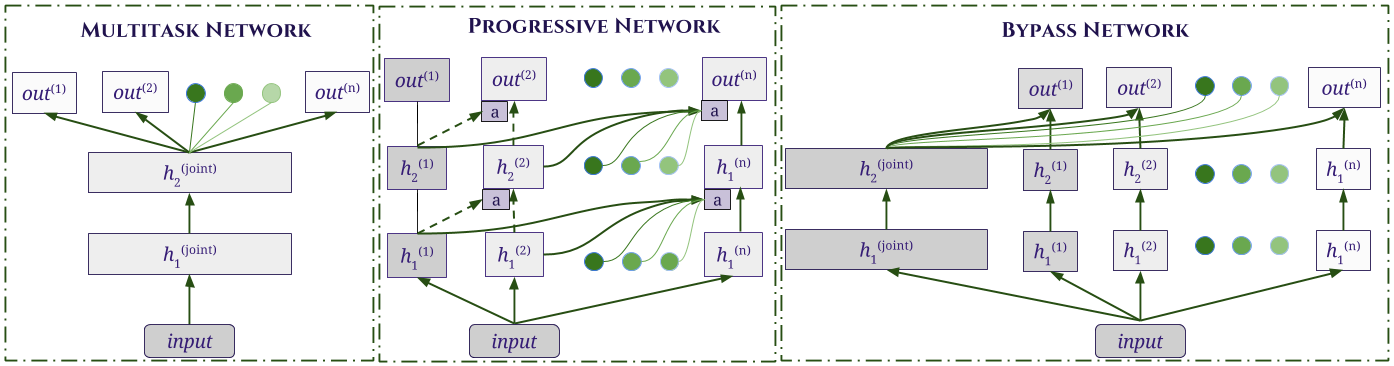
\includegraphics[width=\textwidth]{Images/robust_architectures.png}
  \caption{Left panel depicts a standard multitask architecture. Center panel depicts a progressive architecture. Dotted lines indicate frozen weights. Right depicts our proposed bypass architecture. Note that terms such as ``input'' and ``h'' above denote rows of neurons and not single neurons.}
  \label{fig:arch}
\end{figure}
\subsubsection{Random Forests}
Random forests \cite{breiman2001random} are an ensemble prediction method, where individual decision trees are trained on subsampled subsets of the original dataset. The results for individual trees are averaged to provide the output for the entire system. Random forests are currently widely used in the pharmaceutical industry for QSAR tasks \cite{svetnik2003random}.

We train RF models with 100 trees each, and with
$m/3$ descriptors used at each node, where $m$ is the
number of features in the AP,DP descriptors (using hyperparameters from previous work \cite{ma2015deep}). Tree nodes with 5 or fewer molecules are not split further.  We use the random-forest implementation from Scikit-Learn \cite{pedregosa2011scikit}, but through the DeepChem API for convenience.

\subsubsection{Singletask Architecture}

Singletask deep networks train a separate multilayer neural network for each learning task in the dataset collection. The model for each task is trained separately using backpropagation on the dataset for that task.

\subsubsection{Multitask Architecture}
Multitask deep networks train a joint representation of input datapoints shared for all learning tasks. This shared joint representation is fed into a separate linear model for each dataset in a dataset collection. The entire model is trained end-to-end on training data using backpropagation. The left panel in Figure~\ref{fig:arch} provides a graphical representation of the architecture. Detailed mathematical descriptions have been provided in previous works \cite{ma2015deep, ramsundar2015massively}.

\subsubsection{Progressive Architecture}
The problem of training models capable of solving many tasks is shared by many applications in machine-learning. The progressive neural network architecture \cite{rusu2016progressive} proposes a general solution to this problem by allotting each learning task an independent column of weights. However, the column for task $i$ can refer to all the weights for tasks $1,\dotsc, i-1$ through nonlinear ``adapter'' connections. Progressive networks are trained one task at a time. When task $i$ is training, only the weights in column $i$ are updated. The weights from previous tasks are frozen and may be referred to by the current column but not updated. See the middle panel Figure~\ref{fig:arch} for a graphical depiction of progressive networks, with full detail in the original paper \cite{rusu2016progressive}.

The major drawback of progressive architectures is that the total number of learnable parameters for task $i$ scales linearly with $i$, due to connections to previously learned weights for tasks $1,\dotsc,i-1$. Consequently, for a dataset with $N$ tasks, the total memory requirement scales as $O(N^2)$. For pharmaceutical dataset collections with potentially hundreds of assays, this memory requirement quickly becomes burdensome. Furthermore, the progressive architecture imposes an ordering upon the available tasks. This ordering is often not meaningful for biochemical datasets. For example, a kinase dataset collection may not have a natural notion of which kinase comes first and which comes second in the ordering.

Despite these issues, progressive networks have demonstrated strong results on challenging reinforcement learning and robotics tasks, so we decided to implement and evaluate the effectiveness of progressive architectures for drug-discovery datasets.

\subsubsection{Bypass Architecture}

Progressive architectures allow for each task to have independent nonlinear transformations. The multitask architecture lacks this property, which may render multitask architectures weak on dataset collections with very different tasks. At the same time, progressive architectures lack the shared learnable representations which render multitask architectures powerful. Consequently, we experiment with a bypass architecture that merges the per-task indepedent nonlinearities of progressive networks and the shared learnable layers of multitask networks. The bypass architecture has shared joint layers like the multitask architectures, but also has an independent column of weights which "bypass" the shared representation for each task. However, unlike the progressive architecture, the independent weights for a given task may not interact with the weights for other tasks. This decision prevents the memory growth of progressive networks and also removes the artificial ordering implicit in progressive architectures. See rightmost panel in Figure~\ref{fig:arch} for a depiction of bypass architectures.

\subsubsection{Model Evaluation Metrics}

Model performance is evaluated by using the squared Pearson correlation coefficient ($R^2$) \cite{ma2015deep}. For multitask models, we consider the mean Pearson $R^2$ over all tasks present in the dataset. Since the mean performance only gives a rough sense of relative performance of models, we consider other metrics which measure performance against a random-forest baseline. First, we compute the fraction of learning tasks where performance is improved relative to the random-forest baseline. Past work has noted that multitask models don't offer consistent improvements (many tasks improve performance, but some do worse as well) \cite{ramsundar2015massively}. Computing the fraction improved allows us to understand the failure modes of deep architectures relative to baseline methods. We also compute the largest per-task $R^2$ increase and decrease of deep models compared to random-forest baselines.

These metrics are meant to measure the ``robustness'' of deep-learning architectures. Namely, a robust deep-learning architecture should always outperform baseline methods. While this ideal is not achievable with current architectures, our goal is to evaluate current deep architectures for their degrees of robustness. We propose that robustness is a general principle for proposed architectures, and should be considered in future algorithmic work as a guiding principle.

We also consider inter-task correlations within the raw datasets. Previous work has indicated that multitask learning leverages correlations between tasks in a dataset collection. To provide a rough measure of inter-task correlation, we plot histograms of all pairwise Pearson $R^2$ scores between tasks in a dataset collection. Histograms with large peaks at $0$ indicate that many tasks are uncorrelated with one another; histograms with large peaks at positive values indicate stronger inter task correlations. Note that this visualization is only meaningful for dense datasets; every datapoint has to have a label for every task.

\subsection{Experimental Results}

In this section, we report performance of random forests, multitask networks, progressive networks, and bypass networks trained on the Kaggle, Factors, Kinase and UV dataset collections. Model hyperparameters were tuned on validation sets with a combination of manual hyperparameter tuning and random hyperparameter search \cite{bergstra2012random}. 

\subsubsection{Kaggle}

\begin{table}[h]
    \centering
    \begin{tabular}{ |c|c|c|c| } 
    \hline
    & Mean training $R^2$ & Mean validation $R^2$ & Mean test $R^2$ \\
    \hline
    \textbf{Multitask} & $0.793 \pm 0.005$ & $0.467 \pm 0.014$ & $0.468 \pm 0.012$  \\
    \hline
    \textbf{Progressive} & $0.887 \pm 0.015$ & $0.436 \pm 0.022$ & $0.432 \pm 0.016$  \\
    \hline
    \textbf{Bypass} & $0.843 \pm 0.004$ & $0.454 \pm 0.012$ & $0.456 \pm 0.012$  \\
    \hline
    \textbf{Singletask} & $0.942 \pm 0.002$ & $0.450 \pm 0.009$ &  $0.448 \pm 0.009$ \\
    \hline
    \textbf{Random Forest} & $0.941\pm 0.000$ & $0.423 \pm 0.008$ & $0.428\pm 0.007$  \\
    \hline
    \end{tabular}
    \caption{Model performance on Kaggle Collection. All experiments repeated 3 times with different choice of random seed. Standard deviations are means across per-task standard deviations over trials.}
    \label{tab:kaggle}
\end{table}

\begin{figure}[H]
  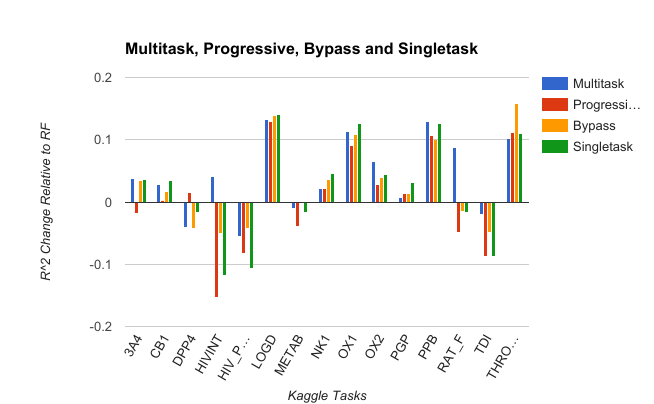
\includegraphics[width=.9\textwidth]{Images/Kaggle_imp.png}
  \caption{Change in performance relative to random forests on Kaggle collection.}
  \label{fig:kaggle-imp}
\end{figure}
\begin{table}[h]
    \centering
    \begin{tabular}{ |c|c|c|c| } 
    \hline
     & Fraction Improved (vs RF) & Largest task $R^2$ drop & Largest task $R^2$ gain \\ 
    \hline
    \textbf{Multitask} & 11/15 & -0.055 & 0.133  \\
    \hline
    \textbf{Progressive} & 9/15 & -0.153 & 0.130  \\
    \hline
    \textbf{Bypass} & 9/15 & -0.050 & 0.157  \\
    \hline
    \textbf{Singletask} & 9/15 & -0.117 & 0.141  \\
    \hline
    \end{tabular}
    \caption{Performance relative to RF baseline on Kaggle test sets.}
    \label{tab:kaggle-comp}
\end{table}

The Kaggle collection serves as a proof of concept that our contributed multitask DeepChem implementation is capable of recapitulating results from the literature \cite{ma2015deep}. Table~\ref{tab:kaggle} reports mean train, validation, and test $R^2$ values for all models on the Kaggle collection. Notably, the singletask and multitask deep architectures achieve performance quantitatively similar to previously reported work, differing only by a couple percentage points (but within previously reported performance ranges for deep networks on this collection). The multitask deep networks offer the strongest validation and test performance of all models tested on the Kaggle collection.

All models overfit the training sets, with mean train $R^2$ significantly higher than mean validation and test $R^2$. Surprisingly, the multitask networks overfit the least, suggesting that the multitask effect acts partially as a regularizer controlling the degree of overfitting. By comparison, both singletask deep networks and random forests have considerably higher training $R^2$ suggesting a greater degree of overfit compared to multitask models. The progressive networks offer comparable performance to random forests, but seem not to perform as well as other deep architectures. The bypass networks behave more similarly to multitask architectures, with strong validation and test performance, but with greater overfitting on the training set, suggesting that the independent bypass layers may harm as well as help.

Table~\ref{tab:kaggle-comp} evaluates the robustness of all deep learning models compared to random forest baselines. Multitask networks perfomed quite robustly with 11 of 15 tasks improved, and worst-case $R^2$ drop of $-.055 R^2$. The bypass networks, singletask, and progressive networks all succeeded in improving 9 of 15 tasks. The progressive and singletask networks suffer more severe per-task $R^2$ drops. Figure~\ref{fig:kaggle-imp} plots the per-task improvement for each model on the Kaggle collection. 

\subsubsection{Factors}
\begin{table}[H]
    \centering
    \begin{tabular}{ |c|c|c|c| } 
    \hline
     & Mean training $R^2$ & Mean validation $R^2$ & Mean test $R^2$ \\
    \hline
    \textbf{Multitask} & $0.941 \pm 0.003$ & $0.517 \pm 0.014$ & $0.424 \pm 0.006$ \\
    \hline
    \textbf{Progressive} & $0.935 \pm 0.001$ & $0.499 \pm 0.001$ & $0.409 \pm 0.005$  \\
    \hline
    \textbf{Bypass} & $0.949 \pm 0.001$ & $0.508 \pm 0.004$ & $0.410 \pm 0.001$ \\
    \hline
    \textbf{Singletask} & $0.954 \pm 0.000$ & $0.504 \pm 0.005$ & $0.393 \pm 0.003$  \\
    \hline
    \textbf{Random Forest} & $0.949 \pm 0.000$ & $0.466 \pm 0.005$ & $0.412 \pm 0.006$ \\
    \hline
    \end{tabular}
    \caption{Model performances on Factors Collection. All experiments repeated 3 times with different choice of random seed. Standard deviations are means across per-task standard deviations over trials.}
    \label{tab:factors}
\end{table}

\begin{figure}[H]
  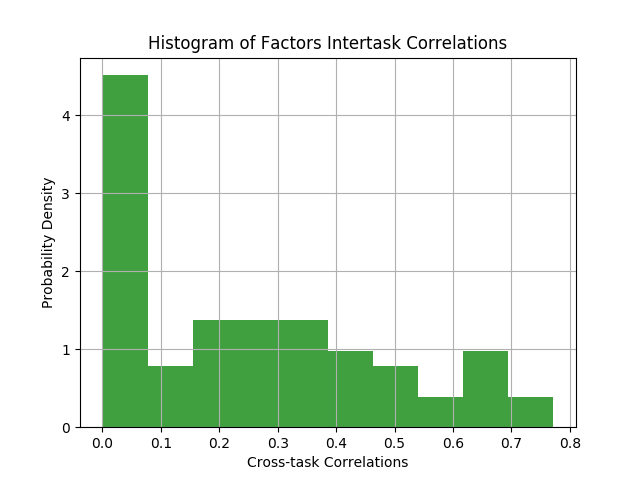
\includegraphics[width=.75\textwidth]{Images/Factors_correlations.png}
  \caption{Histogram of correlations between Factors tasks. The Pearson $R^2$ is computed for each pair of tasks in collection. The histogram displays all computed correlations.}
  \label{fig:factors-corrs}
\end{figure}

\begin{figure}[H]
  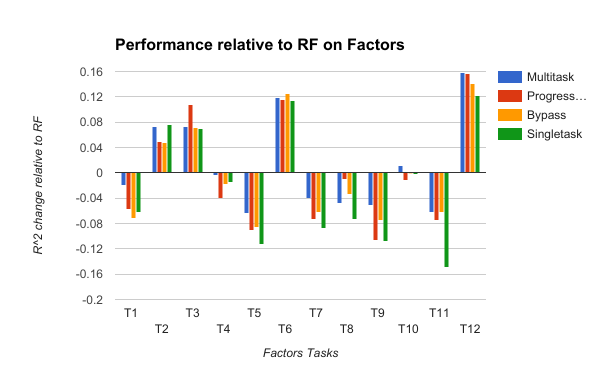
\includegraphics[width=.9\textwidth]{Images/Factors_imp.png}
  \caption{Change in performance relative to random forests on Factors collection. }
  \label{fig:factors-imp}
\end{figure}


\begin{table}[h]
    \centering
    \begin{tabular}{ |c|c|c|c| } 
    \hline
     & Fraction Improved (vs RF) & Largest task $R^2$ drop & Largest task $R^2$ gain \\ 
    \hline
    \textbf{Multitask} & 5/12 & -0.064 & .158  \\
    \hline
    \textbf{Progressive} & 4/12 & -0.108 & .157  \\
    \hline
    \textbf{Bypass} & 4/12 & -.087 & .141 \\
    \hline
    \textbf{Singletask} & 4/12 & -.150 &  .122 \\
    \hline
    \end{tabular}
    \caption{Performance relative to RF baseline on Factors test sets. All experiments repeated 3 times with different choice of random seed. Standard deviations are means across per-task standard deviations over trials.}
    \label{tab:factors-comp}
\end{table}

The Factors collection measures IC50 of inhibition for 12 serine proteases. The measurements for the Factors collection are dense; each molecule is measured in every assay. Figure~\ref{fig:factors-corrs} reports the histogram of correlations between various Factors tasks. While many Factors tasks are effectively uncorrelated, a large proportion of tasks have moderate to high inter-task correlations.

Results for trained models on this collection are reported in Table~\ref{tab:factors} and visualized in Figure~\ref{fig:factors-imp}. The multitask networks achieve the best mean validation and test $R^2$, with the bypass models following closely behind. The Factors collection has only 1500 compounds, compared to the 100 thousand in the Kaggle collection, so perhaps unsurprisingly all models overfit much more heavily than for the Kaggle collection. The multitask effect does not seem to regularize performance on this collection as effectively.

Table~\ref{tab:factors-comp} provides measurements of robustness for the deep models relative to the random forest baseline, and Figure~\ref{fig:factors-imp} provides a graphical representation of model improvement. Perhaps due to the large number of tasks with low correlations, the multitask networks succeed in improving only 5 of 12 tasks. However, tasks that are improved have large boosts in accuracy, while the worst-case drop of $-.064 R^2$ is relatively small. The Progressive, singletask, and bypass models each improve $4$ of $12$ assays, but have worst-case drops larger than for the multitask models.

\subsubsection{Kinase}
\begin{table}[H]
    \centering
    \begin{tabular}{ |c|c|c|c| } 
    \hline
     & Mean training $R^2$ & Mean validation $R^2$ & Mean test $R^2$ \\ 
     %comment MT: R^2
    \hline
    \textbf{Multitask} & $0.897 \pm 0.002$ & $0.301 \pm 0.012$ & $0.238 \pm 0.010$  \\
    \hline
    \textbf{Progressive} & $0.833 \pm 0.012$ & $0.284 \pm 0.006$ & $0.207 \pm 0.001$  \\
    \hline
    \textbf{Bypass} & $0.941 \pm 0.003$ & $0.285 \pm 0.009$ & $0.224 \pm 0.008$  \\
    \hline
    \textbf{Singletask} & $0.951 \pm 0.004$ & $0.284 \pm 0.011$ & $0.229 \pm 0.010$  \\
    \hline
    \textbf{Random Forest} & $0.941 \pm 0.001$ & $0.263 \pm 0.011$ & $0.208 \pm 0.001$  \\
    \hline
    \end{tabular}
    \caption{Model performance on Kinase Collection. All experiments repeated 3 times with different choice of random seed. Standard deviations are means across per-task standard deviations over trials.}
    \label{tab:kinase}
\end{table}
\begin{figure}[H]
  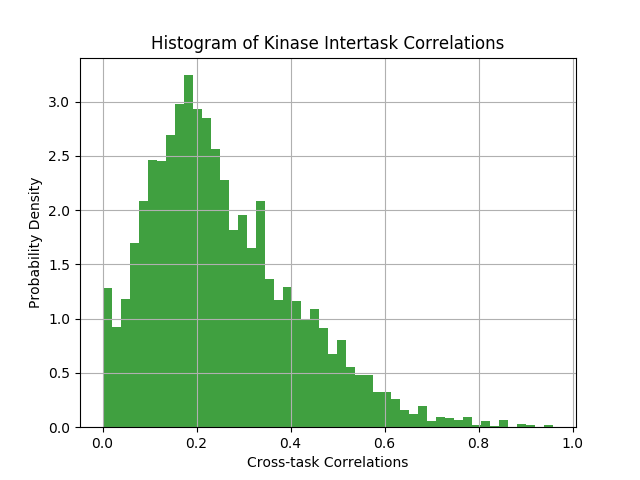
\includegraphics[width=.75\textwidth]{Images/Kinase_correlations.png}
  \caption{Histogram of correlations between Kinase tasks. The Pearson $R^2$ is computed for each pair of tasks in collection. The histogram displays all computed correlations.}
  \label{fig:kinase-corrs}
\end{figure}
\begin{figure}[H]
  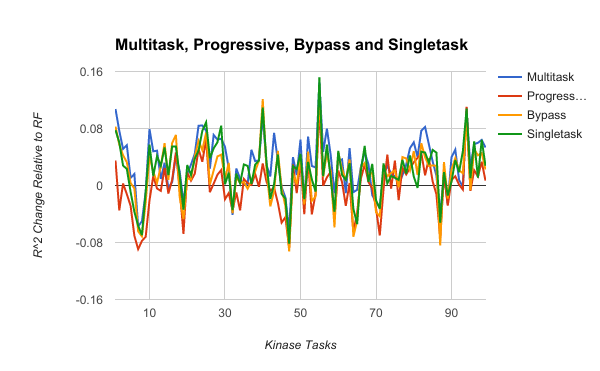
\includegraphics[width=.9\textwidth]{Images/Kinase_imp.png}
  \caption{Change in performance relative to random forests on Kinase collection. Separate lines for each model type are used instead of bars due to large number of tasks.}
  \label{fig:kinase-imp}
\end{figure}

\begin{table}[h]
    \centering
    \begin{tabular}{ |c|c|c|c| } 
    \hline
     & Fraction Improved (vs RF) & Largest task $R^2$ drop & Largest task $R^2$ gain \\ 
    \hline
    \textbf{Multitask} & 79/99 & -0.064 & 0.144  \\
    \hline
    \textbf{Progressive} & 53/99 & -0.089 & 0.111  \\
    \hline
    \textbf{Bypass} & 74/99 & -0.093 & 0.131  \\
    \hline
    \textbf{Singletask} & 78/99 & -0.082 & 0.152  \\
    \hline
    \end{tabular}
    \caption{Performance relative to RF baseline on Kinase test sets.}
    \label{tab:kinase-comp}
\end{table}

The Kinase collection consists of 2500 compounds tested against 99 kinase assays. This collection like Factors (and unlike Kaggle) is dense, with all molecules measured in all assays.  Figure~\ref{fig:kinase-corrs} reports the histogram of correlations between various Kinase tasks, displaying that most tasks have moderate to strong correlations with other tasks in collection.

Table~\ref{tab:kinase} reports mean train, validation, and test $R^2$ of trained models on this collection and Figure~\ref{fig:kinase-imp} displays graphically performance relative to random forest baseline. Multitask models demonstrate the strongest performance on both validation and test sets. Progressive networks again achieve performance similar to random-forests, with the bypass and singletask models offering performance between random forests and multitask architectures. Given the greater number of compounds, the multitask networks once again overfit less severely than singletask deep networks and random forests. Notably, progressive networks appear to underfit this dataset, and achieve the lowest training $R^2$. This underfit is likely due to memory issues; to handle training of progressive networks with 99 tasks (recall that memory usage scales as $O(N^2)$ where $N$ is the number of tasks), we limited the number of hidden nodes per task (per layer) to $50$, which may have reduced the models' explanatory capacity.

Table~\ref{tab:kinase-comp} evaluates the robustness of the deep learning methods relative to the random forest baseline. The multitask networks are quite robust on this collection, providing improvements for 79/99 assays. This broad improvement may be due to the fact that kinase inhibitors are often promiscuous across many kinases \cite{anastassiadis2011comprehensive}, suggesting that shared representations can be easily extracted. (Figure~\ref{fig:kinase-corrs} supports this assertion.) The worst case performance drop of $-.064 R^2$ for multitask models is moderate, suggesting that multitask methods are strong models for Kinase systems. The bypass and singletask models also succeed in offering broad improvement, respectively for 74/99 and 78/99 assays, but with slightly larger worst-case drops of $-.089 R^2$ and $-.082 R^2$ respectively. The progressive models only improve 53/99 assays relative to random forests, possibly due to the model's inability to exploit intertask correlations.

\subsubsection{UV}
\begin{table}[h]
    \centering
    \begin{tabular}{ |c|c|c|c| } 
    \hline
     & Mean training $R^2$ & Mean validation $R^2$ & Mean test $R^2$ \\
    \hline
    \textbf{Multitask} & $0.961 \pm 0.001$ & $0.420 \pm 0.013$ & $0.441 \pm 0.014$  \\
    \hline
    \textbf{Bypass} & $0.903 \pm 0.005$ & $0.396 \pm 0.014$ & $0.421 \pm 0.014$  \\
    \hline
    \textbf{Singletask} & $0.968 \pm 0.002$ & $0.399 \pm 0.012$ & $0.417 \pm 0.013$ \\
    \hline
    \textbf{Random Forest} & $0.961 \pm 0.000$ & $0.404 \pm 0.006$ & $0.428 \pm 0.006$  \\
    \hline
    \end{tabular}
    \caption{Model performance on UV Collection. All experiments repeated 3 times with different choice of random seed. Standard deviations are means across per-task standard deviations over trials. Progressive networks were omitted since models took over a day to train.}
    \label{tab:uv}
\end{table}

\begin{figure}[H]
  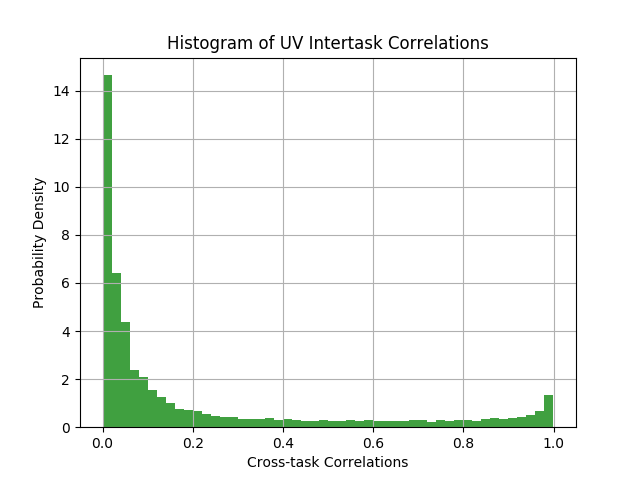
\includegraphics[width=.75\textwidth]{Images/UV_correlations.png}
  \caption{Histogram of correlations between UV tasks. Pearson $R^2$ is computed for each pair of tasks in collection. Histogram displays all computed correlations.}
  \label{fig:uv-corrs}
\end{figure}
\begin{figure}[H]
  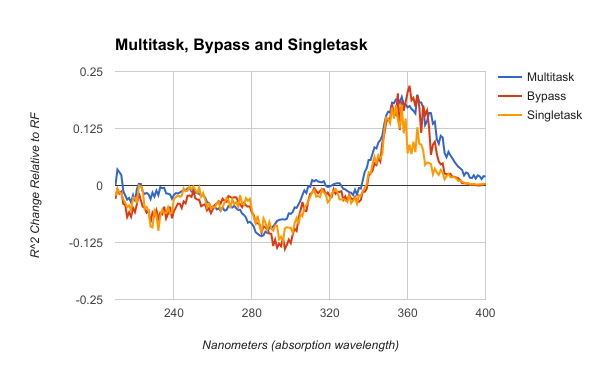
\includegraphics[width=.9\textwidth]{Images/UV_imp.png}
  \caption{Change in performance relative to random forests on UV collection. Separate lines for each model type are used instead of bars due to large number of tasks.}
  \label{fig:uv-imp}
\end{figure}
\begin{table}[h]
    \centering
    \begin{tabular}{ |c|c|c|c| } 
    \hline
     & Fraction improved (vs RF)  & Largest task $R^2$ Drop & Largest task $R^2$ gain \\ 
    \hline
    \textbf{Multitask} & 81/190 &  -.111 & 0.199  \\
    \hline
    \textbf{Bypass} & 60/190 & -0.139 & 0.219  \\
    \hline
    \textbf{Singletask} & 63/190  & -0.122  & 0.177  \\
    \hline
    \end{tabular}
    \caption{Performance relative to RF baseline on UV test sets.}
    \label{tab:uv-comp}
\end{table}


The UV dataset collection consists of roughly 10,000 compounds evaluated over 190 absorption wavelengths (210-400 nm). The UV collection (like the Factors and Kinase collections) is dense, with all molecules measured at all wavelengths. Figure~\ref{fig:uv-corrs} reports the histogram of correlations between various UV tasks. Unlike other collections, most assays are weakly correlated. The small bump at high correlation is due to fact that absorption at nearby wavelengths is highly correlated (absorption at 231nm and 232nm likely have high correlation for example).


Table~\ref{tab:uv} reports mean train, valid, and test $R^2$ values for models on this dataset collection. Multitask models achieve the highest mean validation and test $R^2$, but only by a slight margin. Note that Table~\ref{tab:uv} does not provide numbers for progressive networks. We could not successfully train progressive models on this collection within a day, likely due to the high graph complexity for a progressive architecture with nearly 200 tasks.

Table~\ref{tab:uv-comp} evaluates robustness of trained models relative to the random forest baseline. Notably, multitask models don't succeed in outperforming the random forest baseline on a majority of assays, with only 81 of the
190 datasets improved. As with Factors, the large number of uncorrelated tasks may have contributed to this outcome. The largest worst-case $R^2$ drop is moderate, with $-.111 R^2$ drop observed on one task, but with large performance gains of $0.199$ on the best-improved task. Figure~\ref{fig:uv-imp} shows an interesting pattern, with most assays underperforming the RF baseline, but with a large fraction showing significant improvements over the RF baseline. The improved assays are all adjacent, indicating that the multitask models may perhaps be learning some shared property of the physics at these wavelengths.


\subsubsection{Singletask versus Multitask}
\begin{table}[h]
    \centering
    \begin{tabular}{ |c|c|c| } 
    \hline
     Dataset Collection & Multitask Improved \\ 
    \hline
    \textbf{Kaggle} & 8/15  \\
    \hline
    \textbf{Factors} & 11/12  \\
    \hline
    \textbf{Kinase} & 64/99  \\
    \hline
    \textbf{UV} & 155/190 \\
    \hline
    \end{tabular}
    \caption{Number of tasks improved by multitasking.}
    \label{tab:tasks-improved}
\end{table}

To evaluate the relative improvement due to the multitask effect, as opposed to changes in performance due to deep learning, we evaluated the fraction of tasks where multitask models outperformed singletask models for all collections we consider. Results are displayed in Table~\ref{tab:tasks-improved}. Notably, a majority of assays in all collections show improvement of multitask over singletask, indicating that multitask deep-learning performs better on our assay collections than singletask deep learning.

\subsection{Discussion and Conclusion}

Preliminary studies have demonstrated that multitask deep learning can offer performance improvements over simpler machine-learning techniques for drug-discovery datasets \cite{ma2015deep, ramsundar2015massively}. However, multitask deep networks have yet to achieve a wide degree of adoption across the pharmaceutical and biotechnology industries. Historically, transforming machine learning prototypes into production systems can be challenging. As noted previously, Netflix decided not to use the winning entry in its million dollar recommendation challenge to serve actual customer recommendations \cite{netflixNever}. We hypothesize that two key barriers prevent the widespread adoption of multitask deep networks: First, implementing deep architectures can be a challenging software endeavor. Second, the failure modes of multitask deep networks relative to random forest and singletask baselines remain poorly understood.

This work has aimed to overcome both barriers to entry for deep architectures. To overcome software challenges, we have introduced a high-quality open-source implementation of multitask deep-networks as part of the DeepChem library for open-source drug-discovery \cite{deepchem}. Our implementation makes it easy to build, fit, and evaluate high quality deep-learning models with simple python scripts (see Figure~\ref{fig:code} for a real code example). We also contribute open-source implementations of two new deep-learning architectures to DeepChem. Progressive networks \cite{rusu2016progressive} were first proposed for robust multitask deep learning in robotic and reinforcement learning applications. We also propose a bypass architecture, which aims to serve as a hybrid of multitask and progressive architectures. 

We used our open source DeepChem implementation to test the behavior of our deep architectures across four broad collections of datasets. We demonstrated that the DeepChem implementation can duplicate qualitatively and quantitatively the performance of deep models on the Kaggle collection analyzed previously in the literature \cite{ma2015deep}. We then evaluated the performance of multitask, singletask, progressive, bypass, and random forests across the Factors, Kinase, and UV dataset collections. In particular, since our validation and test splits use time and neighbor-split (known to be challenging for multitask methods), our evaluation constitutes a ``worst-case'' test of multitask performance. Even under these challenging conditions, multitask models offer the strongest mean validation and test set $R^2$ across all evaluated collections. 

To further evaluate model performance, we introduced a set of robustness measurements, which measure the fraction of assays improved by deep architectures relative to random forest baselines. We also considered the worst-case and best-case per-task $R^2$ improvement over all tasks. Multitask architectures are more robust than progressive, singletask, and bypass architectures on these datasets, with a majority of assays improved over RF on the Kaggle and Kinase dataset. On the Factors and UV datasets, fewer assays are improved, likely due to lower inter-task correlations, but some tasks see quite significant improvements and only moderate performance drops elsewhere. Worst-case performance drops are lowest for multitask architectures compared to other deep architectures. Broadly, our robustness analysis suggest that multitask deep-models can offer improvements over random forests for a wide variety of models, and especially in collections with high inter-task correlations. Our work suggests that multitask architectures can be fruitfully applied to many datasets that arise in drug discovery.  

%%% NEW PARAGRAPH

In general, we note that while multitask deep learning provides improvements over random forest methods on average, many assays suffer worse performance compared with the random forest baseline. While the full investigation of these failures is left to future work, we note that the use of obfuscated fingerprints that obscure molecular structures may be limiting the potential of deep learning methods on these datasets. Subsequent work by some of the authors of the present paper has shown that graph convolutional models \cite{duvenaud2015convolutional} implemented in DeepChem can achieve significant boosts in performance over multitask deep networks on the MoleculeNet benchmark suite \cite{wu2017moleculenet}. In the future, it may be interesting to test these graph convolutional methods in collaboration projects on pharmaceutical data. The DeepChem library will hopefully serve to enable such research.

%%% NEW PARAGRAPH

%%% NEW PARAGRAPH

We note that in this paper, we did not attempt to place error bars on the predictions made for individual molecules. The presence of good error bars allows practitioners to reason about the domain of applicability for learned models. However, gauging the confidence of predictions from deep learning models is known to be challenging. There has been significant recent interest in the methods of Bayesian deep learning \cite{kendall2017uncertainties}, which may provide a structured solution to the uncertainty modeling problem. Extending Bayesian deep learning methods to pharmaceutical applications is beyond the scope of the present work however, and we suggest it as a good topic for future work.

%%% NEW PARAGRAPH

Our open-source multitask deep network implementation in DeepChem can help facilitate the broad adoption of deep networks in commercial drug discovery. In particular, we open source our deep learning models for all collections in this paper (along with the associated datasets) to serve as a community resource. We anticipate that our open-source implementation in tandem with our statistical robustness analysis across a broad collection of datasets will facilitate the widespread adoption of multitask deep-learning in the pharmaceutical industry.


\subsection{Acknowledgements}

We would like to thank the Stanford Computing Resources for providing us with access to the Sherlock and Xstream GPU nodes. Thanks to Junshui Ma for help in debugging performance on the Kaggle collection. Thanks to Kevin McCloskey and Patrick Riley from Google for open-sourcing the code that formed the preliminary DeepChem multitask implementation. Thanks to Aarthi Ramsundar for help with diagram construction.

The Pande Group is broadly supported by grants from the NIH (R01 GM062868 and U19 AI109662) as well as gift funds and contributions from Folding@home donors.

We acknowledge the generous support of Dr. Anders G. Fr{\o}seth for our work on machine learning.

B.R. was supported by the Fannie and John Hertz Foundation.

AV, MT, RPS are employees of Merck \& Co., Inc. of Kenilworth, NJ. VSP is a consultant and SAB member of Schrodinger, LLC and Globavir, sits on the Board of Directors of Apeel Inc, Freenome Inc, Omada Health, Patient Ping, Rigetti Computing, and is a General Partner at Andreessen Horowitz.

